%\subsection{Univariate Gaussian}
%
\setbeamercovered{still covered={\opaqueness<1->{0}},again covered={\opaqueness<1->{15}}}
%\begin{frame}[label=varex]{Estimation of a 1-dim Gaussian mean and variance}
%  \vspace{-5pt}
%  \begin{itemize}
%    \item<1-3> \textbf{GOAL}: Bayesian inference of mean $\mu$ and variance $\psi^{-1}$
%    \begin{center}
%      {\def\arraystretch{1.2}
%      \begin{tabular}{c c l}
%        $\displaystyle y_i \iid \N(\mu, \psi^{-1})$ & & Data \\
%        {\color{gray!88}$\displaystyle \mu|\psi \sim \N\big(\mu_0,(\kappa_0\psi)^{-1}\big)$} & & {\color{gray!88}\multirow{2}{*}{Priors}} \\
%        {\color{gray!88}$\displaystyle \psi \sim \Gamma(a_0,b_0)$} & \\
%        $\displaystyle i=1,\dots,n$ & \\
%      \end{tabular}
%      }
%    \end{center}
%    \item<2-3> Substitute $p(\mu,\psi|\by)$ with the mean-field approximation
%    \[
%      q(\mu, \psi) = q_\mu(\mu) q_\psi(\psi).
%    \]
%    \item<3-> From \eqref{eq:meanfieldsoln}, we can work out the solutions 
%    
%    \only<5|handout:0>{
%    \begin{align*}
%      \log \tilde q_\mu(\mu) 
%      &= \E_\psi[\log p(\by|\mu,\psi)] + \E_\psi[\log p(\mu|\psi)] + \const \\[0.5em]
%    \log \tilde q_\psi(\psi) 
%    &= \E_\mu[\log p(\by|\mu,\psi)] + \E_\mu[\log p(\mu|\psi)] + \log p(\psi) \\
%    &\phantom{==} + \const
%    \end{align*}
%    }
%    
%    \vspace{-3pt}
%    \begin{gather*}
%      \uncover<6->{
%      \hspace{-12pt}\tilde q_\mu(\mu) \equiv \N \left(\frac{\kappa_0 \mu_0 + n\bar y}{\kappa_0 + n}, \frac{1}{(\kappa_0 + n)\E_q[\psi]} \right)}
%      \uncover<7->{
%      \ \text{ and } \ \
%      \tilde q_\psi(\psi) \equiv \Gamma(\tilde a, \tilde b) \\[0.5em]
%      \hspace{-12pt}\tilde a = a_0 + \half[n] \hspace{1.1cm} \tilde b = b_0 + \half \E_q\Big[ {\textstyle\sum_{i=1}^n} (y_i - \mu)^2 + \kappa_0(\mu - \mu_0)^2 \Big]
%      }
%    \end{gather*}
%  \end{itemize}
%  
%  \only<4-|handout:0>{
%  \begin{textblock*}{0.8\textwidth}(1.35cm,0.215\textheight)
%    \begin{block}{}
%      \begin{itemize}
%        \item Under the mean-field restriction, the solution to $\argmax_q \cL(q)$ is
%        \begin{align*}
%          \tilde q_j(\bz^{(j)}) \propto \exp\big(\E_{-j}[\log p(\by,\bz)]\big)
%          \rlap{\hspace{1.3cm}(1)}
%        \end{align*}
%        for $j \in \{1,\dots,m\}$.  
%      \end{itemize}
%    \end{block}
%  \end{textblock*}
%  }
%
%%  \begin{textblock*}{3cm}(.982\textwidth,1.04\textheight)%
%%    \hyperlink{cavi}{\beamerbutton{back}}      
%%  \end{textblock*}
%
%\end{frame}
%
%\begin{frame}{Estimation of a 1-dim Gaussian mean and variance (cont.)}
%  \vspace{-5pt}
%%  \only<1>{
%%    \begin{center}
%%      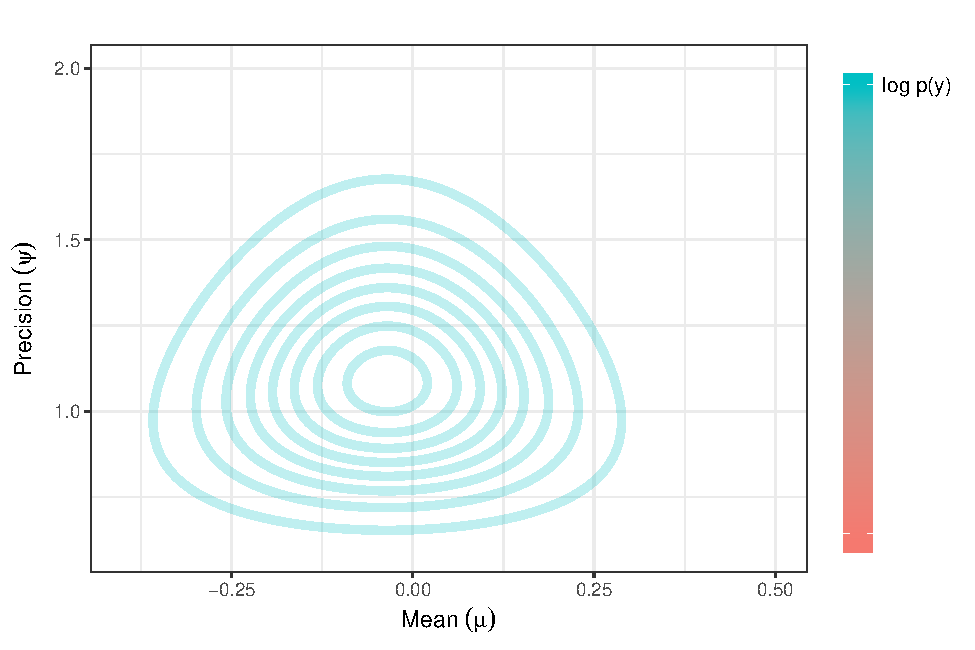
\includegraphics[scale=0.7]{figure/vbupdate}
%%    \end{center}
%%  } 
%  \only<1|handout:1>{
%    \begin{center}
%      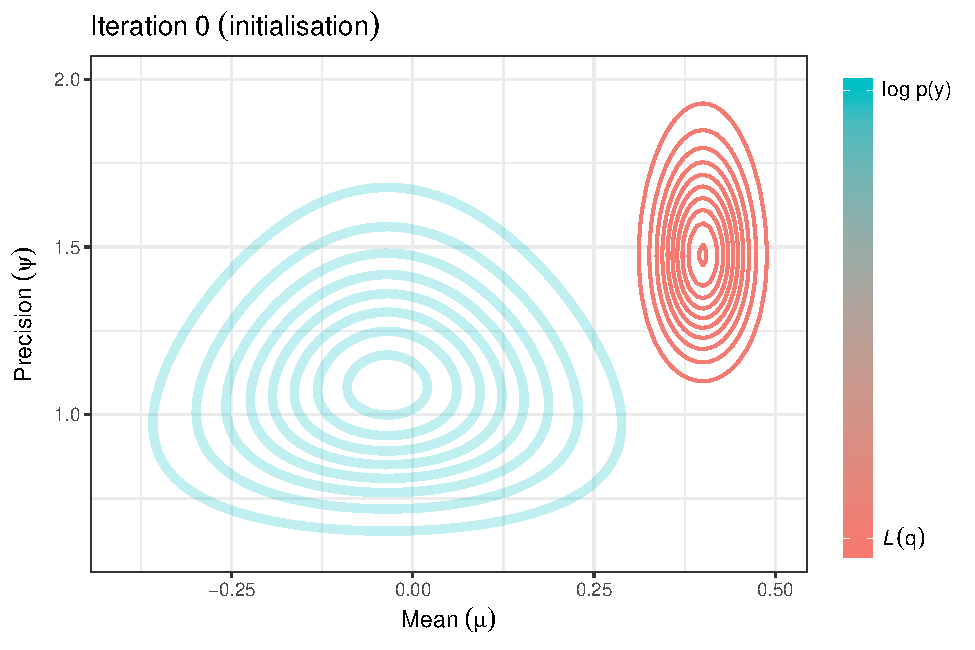
\includegraphics[scale=0.7]{figure/vbupdate_7}
%    \end{center}
%  } 
%  \only<2|handout:2>{
%    \begin{center}
%      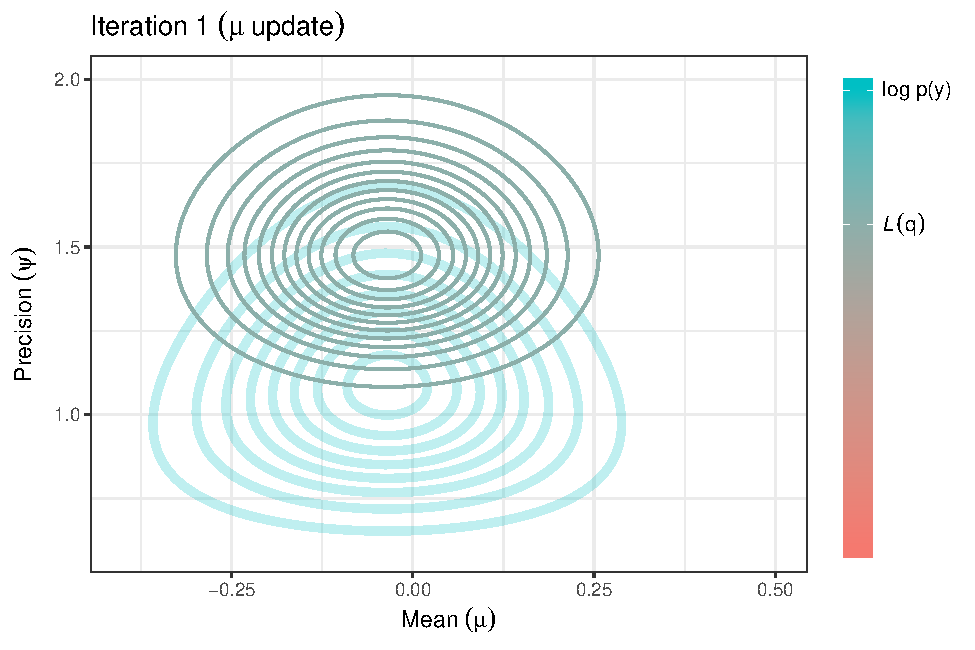
\includegraphics[scale=0.7]{figure/vbupdate_1}
%    \end{center}
%  } 
%  \only<3|handout:3>{
%    \begin{center}
%      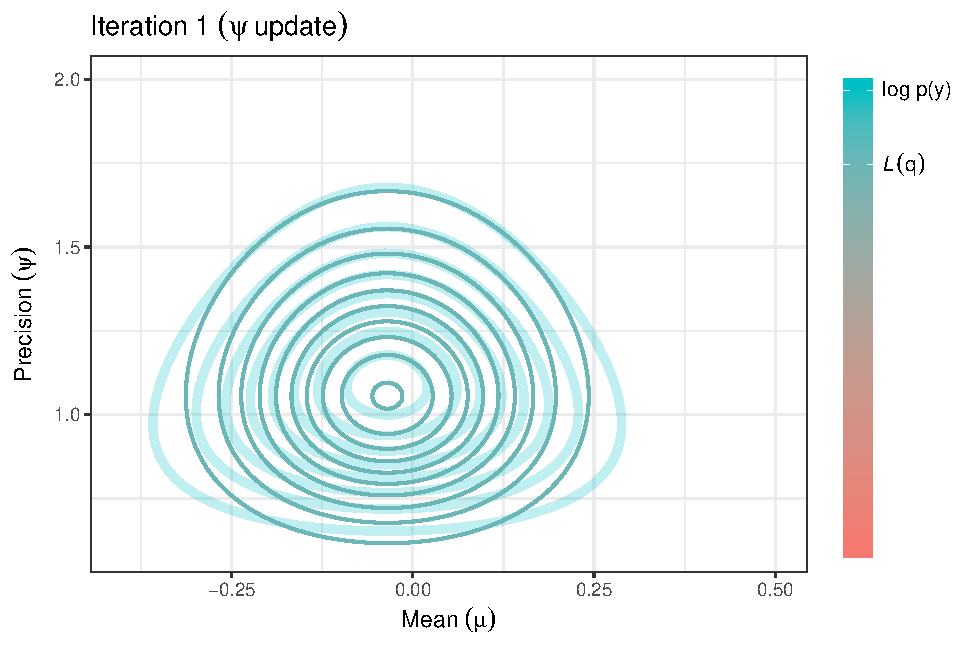
\includegraphics[scale=0.7]{figure/vbupdate_2}
%    \end{center}
%  } 
%  \only<4|handout:4>{
%    \begin{center}
%      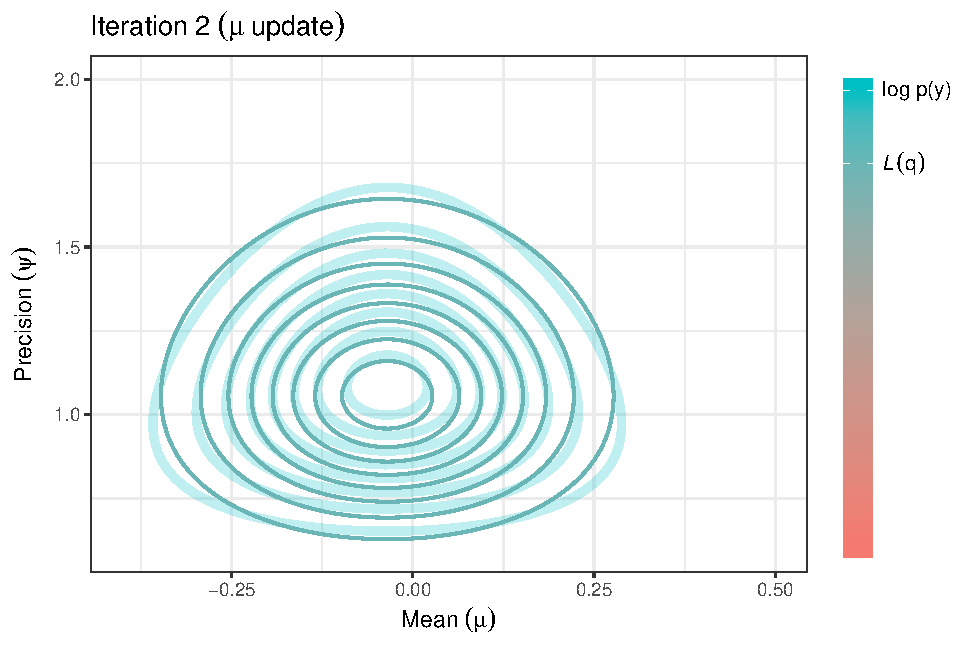
\includegraphics[scale=0.7]{figure/vbupdate_3}
%    \end{center}
%  } 
%  \only<5|handout:5>{
%    \begin{center}
%      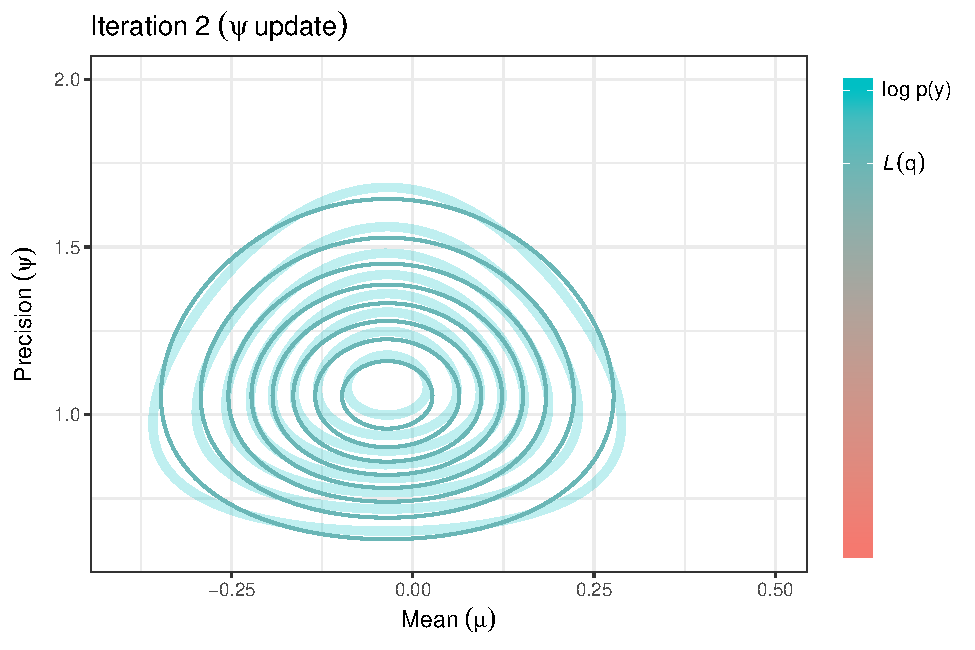
\includegraphics[scale=0.7]{figure/vbupdate_4}
%    \end{center}
%  } 
%  
%%  \begin{textblock*}{3cm}(.982\textwidth,1.04\textheight)%
%%    \hyperlink{cavi}{\beamerbutton{back}}      
%%  \end{textblock*}
%\end{frame}
%
%\begin{frame}{Comparison of solutions}
%  
%  {\centering
%  \begin{minipage}{0.45\linewidth}
%    \underline{Variational posterior}
%    {\small
%    \begin{align*}
%      &\mu \sim \N \left(\frac{\kappa_0 \mu_0 + n\bar y}{\kappa_0 + n}, \frac{1}{(\kappa_0 + n)\E[\psi]} \right) \\
%      &\psi \sim \Gamma\left(a_0 + \half[n], b_0 + \half c\right) \\
%      &c = \E\Big[ {\sum_{i=1}^n} (y_i - \mu)^2 + \kappa_0(\mu - \mu_0)^2 \Big]
%    \end{align*}}
%  \end{minipage}
%  \hspace{6mm}
%  \begin{minipage}{0.45\linewidth}
%    \underline{True posterior}
%    {\small
%    \begin{align*}
%      &\mu|\psi \sim \N \left(\frac{\kappa_0 \mu_0 + n\bar y}{\kappa_0 + n}, \frac{1}{(\kappa_0 + n)\psi} \right) \\
%      &\psi \sim \Gamma\left(a_0 + \half[n], b_0 + \half c' \right) \\
%      &c' = {\sum_{i=1}^n} (y_i - \bar y)^2 + \frac{\kappa_0}{\kappa_0 + n}(\bar y - \mu_0)^2
%    \end{align*}}    
%  \end{minipage}}
%  
%  \begin{itemize}
%    \item $\Cov(\mu,\psi) = 0$ by design in VI solutions.
%    \item For this simple example, it is possible to decouple and solve explicitly.
%    \item VI solutions leads to unbiased MLE if $\kappa_0 = \mu_0 = a_0 = b_0 = 0$.
%  \end{itemize}
%\end{frame}